\section{Trapezregel}
\label{sec:trapezregel}

\subsection{Herleitung}
\label{sec:herleitung}

\begin{figure}[h]
    \centering
    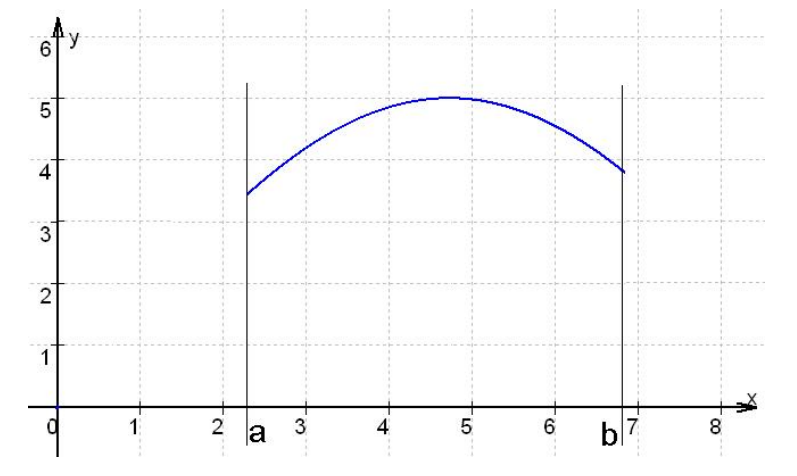
\includegraphics[width=8cm]{Bilder/keplersche_fassregel_funktion.png}
    \caption{Keplersche Fassregel \cite{skript}}    
    \label{fig:keplersche_fassregel}
\end{figure}

Wir betrachten eine Funktion $f$, deren Schaubild im gewünschten Intervall $I = [a, b]$ in \autoref{fig:sehnentrapeze} gezeigt ist.

\begin{figure}[!tbp]
    \centering
    \begin{minipage}[b]{0.4\textwidth}
        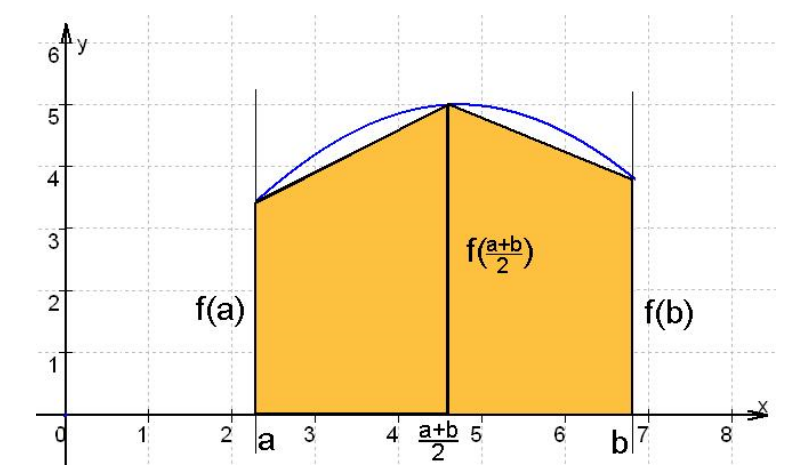
\includegraphics[width=8cm]{Bilder/sehnentrapeze.png}
      \caption{Sehnentrapeze für die anstehende Rechnung}
    \end{minipage}
    \hfill
    \begin{minipage}[b]{0.4\textwidth}
        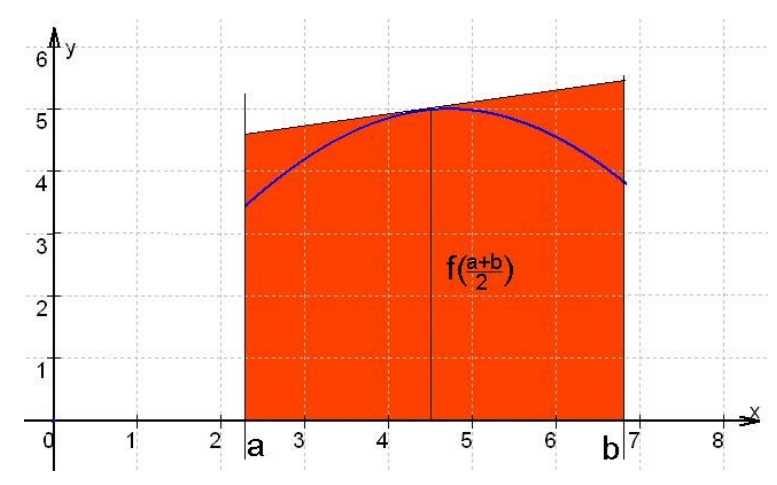
\includegraphics[width=8cm]{Bilder/sehnentrapez_addiert.png}
      \caption{Tangententrapez  \cite{skript}}
    \end{minipage}
    \label{fig:sehnentrapeze}
  \end{figure}
\subsection*{A. Die zwei Sehnentrapeze}

Zur Flächenberechnung zeichnen wir zwei Sehnentrapeze in das gegebene Schaubild, wie in \autoref{fig:sehnentrapeze} zu sehen ist. Für die Fläche eines Trapezes gilt:
\[
A_{\text{Trapez}} = \frac{a + c}{2} \cdot h = m \cdot h
\]
Übertragen auf die beiden Sehnentrapeze ergibt sich die Gesamtfläche $S$ als:
\[
S = \frac{b - a}{2} \cdot \left(\frac{f(a)}{2} + f\left(\frac{a + b}{2}\right) + \frac{f(b)}{2}\right)
\]
Dies lässt sich umschreiben zu:
\[
S = \frac{b - a}{2} \cdot \left(\frac{f(a)}{2} + f\left(\frac{a + b}{2}\right) + \frac{f(b)}{2}\right)
\]

\subsection*{B. Das Tangententrapez}

Nun legen wir ein weiteres Tangententrapez in das Schaubild, wie in \autoref{fig:sehnentrapeze} dargestellt. Nach der Trapezformel ergibt sich:
\[
T = f\left(\frac{a + b}{2}\right) \cdot (b - a)
\]
Da wir doppelt so viele Sehnentrapeze wie Tangententrapeze haben, gewichten wir die Flächen entsprechend. Die Gesamtfläche $I[f]$ nähert sich durch:
\[
I[f] \approx A = \frac{1}{3} \cdot (2S + T)
\]
Dies lässt sich weiter vereinfachen zu:
\[
A = \frac{b - a}{6} \cdot \left(f(a) + 4 \cdot f\left(\frac{a + b}{2}\right) + f(b)\right)
\]

\subsection*{Die Keplersche Fassregel}

Ist die Funktion $f$ auf dem Intervall $I = [a, b]$ stetig, so gilt die Keplersche Fassregel:
\[
I[f] \approx A = \frac{b - a}{6} \cdot \left(f(a) + 4 \cdot f\left(\frac{a + b}{2}\right) + f(b)\right)
\]
Dabei ist zu beachten, dass die Keplersche Fassregel nur dann gute Näherungswerte liefert, wenn sich die Funktion im betrachteten Intervall durch eine Parabel annähern lässt. Daher ist es ratsam, das Intervall $[a, b]$ in viele kleine, gleich große Teilintervalle zu unterteilen und die Keplersche Fassregel auf jedes Teilintervall anzuwenden. Diese Methode wird im nächsten Abschnitt besprochen, in dem die summierten Regeln behandelt werden. \cite{skript}

\subsection{Fehlerabschätzung}
\label{sec:fehlerabschätzung}

Für die Fehlerberechnung brauchen wir mehrere Schritte:
\subsection*{Definition des Fehlers}
Der Fehler wird definiert als die Breite des Konfidenzintervalls, die berechnet wird als:
\[
\text{Breite} = 2 \cdot c \cdot \frac{\sigma}{\sqrt{n}}
\]

\subsection*{Berechnung des Standardfehlers}
Der Standardfehler (SE) des Mittelwerts wird berechnet als:
\[
SE = \frac{\sigma}{\sqrt{n}}
\]

\subsection*{Schätzung des Fehlers}
Die Fehlerabschätzung kann dann wie folgt berechnet werden:
\[
\text{Fehlerabschätzung} = c \cdot SE
\]

\subsection*{Iterative Fehlerabschätzung}
Um die Auswirkungen verschiedener Stichprobengrößen zu untersuchen, kann das Konfidenzintervall für unterschiedliche Stichproben berechnet werden. Die Variabilität in der Breite der Intervalle gibt Aufschluss über die Stabilität der Schätzungen.

\subsection*{Interpretation}
Ein kleiner Fehler zeigt an, dass das Konfidenzintervall eine präzise Schätzung des wahren Mittelwerts bietet. Ein größerer Fehler deutet auf mögliche Unsicherheiten in den Daten oder eine unzureichende Stichprobengröße hin.


\subsection{Vertrauensniveau $\gamma$}
\label{sec:vertrauensniveau}
Das Vertrauensniveau \(\gamma\) ist ein Konzept, das angibt, wie sicher wir sind, dass ein berechnetes Konfidenzintervall den wahren Wert eines Parameters enthält. Es wird häufig als Dezimalzahl zwischen 0 und 1 dargestellt, wobei typische Werte 0.95 (95\%) und 0.99 (99\%) sind.

\begin{itemize}
    \item \textbf{Einfluss auf die Breite des Intervalls:} Ein höheres Vertrauensniveau führt zu einem breiteren Konfidenzintervall. Das bedeutet, dass wir mit größerer Sicherheit sagen können, dass der wahre Wert in diesem Intervall liegt. Ein niedrigeres Vertrauensniveau hingegen führt zu einem schmaleren Intervall, was die Schätzung präziser macht, aber auch das Risiko erhöht, dass der wahre Wert außerhalb liegt.
    
    \item \textbf{Berechnung:} Das Vertrauensniveau wird verwendet, um kritische Werte zu bestimmen, die notwendig sind, um das Konfidenzintervall zu berechnen. Beispielsweise erfordert ein 95\%-Konfidenzintervall die Verwendung eines spezifischen z-Werts aus der Normalverteilung, um den Bereich zu bestimmen, in dem der wahre Parameter mit 95\%iger Sicherheit liegt.
\end{itemize}
Insgesamt ist das Vertrauensniveau \(\gamma\) ein zentrales Element statistischer Analysen. Es ermöglicht uns, die Unsicherheit in unseren Schätzungen zu quantifizieren und zu kommunizieren.

\subsection{Alternativen zur Trapezregel} 
\label{sec:alternativen}
Es gibt mehrere alternative Methoden zur numerischen Integration, die oft genauer oder effizienter sind als die Trapezregel. Hier sind einige gängige Alternativen:

\subsection*{Simpsonregel}
Die \textbf{Simpsonregel} ist eine weit verbreitete Methode zur numerischen Integration, die die Fläche unter einer Kurve mithilfe von Parabeln approximiert. Sie ist genauer als die Trapezregel, insbesondere bei glatten Funktionen. Es gibt zwei Hauptvarianten:

\begin{itemize}
    \item \textbf{Einfaches Simpsonverfahren}: Hierbei wird das Intervall in eine gerade Anzahl von Teilintervallen unterteilt, und die Fläche unter der Funktion wird durch Parabeln approximiert.
    \[
    \int_{a}^{b} f(x) \,dx \approx \frac{h}{3} \left( f(a) + 4f\left(\frac{a+b}{2}\right) + f(b) \right)
    \]
    wobei \(h = \frac{b-a}{2}\) die Breite des Intervalls ist.
    
    \item \textbf{Simpson 3/8-Regel}: Diese Methode verwendet drei Teilintervalle und hat eine ähnliche Formel, bietet jedoch höhere Genauigkeit für bestimmte Funktionen.
\end{itemize}

\subsection*{Romberg-Integration}
Die \textbf{Romberg-Integration} kombiniert die Trapezregel mit einer Fehlerabschätzung und verwendet eine extrapolative Technik, um die Genauigkeit zu erhöhen. Sie berechnet die Trapezregel für verschiedene Schrittweiten und verwendet diese Werte, um eine genauere Schätzung zu erhalten. Dies geschieht durch wiederholte Anwendung der Trapezregel und die Verwendung von Richardson-Extrapolation.

\subsection*{Monte-Carlo-Integration}
Die \textbf{Monte-Carlo-Integration} ist eine probabilistische Methode zur numerischen Integration. Sie eignet sich gut für mehrdimensionale Integrale und komplizierte Regionen. Dabei werden zufällige Punkte im Integrationsbereich erzeugt, und die Funktionswerte an diesen Punkten werden zur Schätzung des Integrals verwendet.

\subsection*{Gauss-Quadratur}
Die \textbf{Gauss-Quadratur} ist eine sehr präzise Methode zur numerischen Integration, die spezifische Punkte (Wurzeln) und Gewichte verwendet, um die Integrationsgenauigkeit zu maximieren. Bei der Gauss-Legendre-Quadratur werden die Wurzeln der Legendre-Polynome verwendet, um das Integral zu approximieren.

\[
\int_{a}^{b} f(x) \,dx \approx \sum_{i=1}^{n} w_i f(x_i)
\]
wobei \(w_i\) die Gewichte und \(x_i\) die Wurzeln der Legendre-Polynome sind.

\subsection*{Adaptive Integration}
\textbf{Adaptive Integrationsmethoden} passen die Schrittweite dynamisch an die Funktion an. Bei diesen Methoden wird die Funktion in Abschnitten integriert, und die Intervallbreite wird verringert, wenn die Funktion starke Änderungen aufweist. Ein Beispiel ist die adaptive Simpsonregel.

